\usepackage{fourier}
\usepackage{bbding}
\usepackage{ucll-code}

\usetikzlibrary{shadows,shapes.multipart}

\title{Allocation Methods}
\author{Fr\'ed\'eric Vogels}




\begin{document}

\begin{frame}
  \titlepage
\end{frame}

\begin{frame}
  \frametitle{Overview}
  \begin{itemize}
    \item Different ways to deal with RAM
    \item Trade flexibility for speed
          \begin{itemize}
            \item Flexible but slow
            \item Rigid but fast
          \end{itemize}
    \item In most languages abstracted away as much as possible
    \item In \cpp: crucial to know about the details
  \end{itemize}
\end{frame}

\section{Static Allocation}

\begin{frame}
  \tableofcontents[currentsection]
\end{frame}

\begin{frame}
  \frametitle{Static Allocation}
  \begin{itemize}
    \item Simplest allocation mechanism
    \item Fastest
    \item Most restrictive
    \item Was only available allocation method in first programming language (Fortran, early 1950s)
  \end{itemize}
  \vskip1cm
  \begin{center}
    {\color{red}\Huge\danger}
    \parbox{8cm}{\centering 
      {\color{red}\Huge \textsc{warning}} \\
      Examples that follow are what-ifs \\
      They do not show how really \cpp\ works
    }
    {\color{red}\Huge\danger}
  \end{center}
\end{frame}

\begin{frame}
  \frametitle{How Does It Work?}
  \notrealcpp
  \begin{itemize}
    \item Compiler scans source code for variables
          \begin{itemize}
            \item Parameters, locals, globals, \dots
          \end{itemize}
    \item The compiler assigns a fixed address to each variable
  \end{itemize}
  \code[language=c++14,frame=none]{allocation.cpp}
  \begin{tikzpicture}[overlay,remember picture,allocation/.style={-latex,thick}]
    \coordinate (upperleft) at (6,4);

    \begin{scope}[scale=.5]
      \coordinate (double) at (upperleft);
      \coordinate (int) at ($ (upperleft) + (0,-1) $);
      \coordinate (char) at ($ (upperleft) + (4,-1) $);

      \visible<2->{
        \draw[fill=red!50] (double) rectangle ++(8,-1);
      }

      \visible<3->{
        \draw[fill=green!50] (int) rectangle ++(4,-1);
      }

      \visible<4->{
        \draw[fill=blue!50] (char) rectangle ++(1,-1);
      }

      \draw (upperleft) grid ++(8,-4);
    \end{scope}

    \visible<2>{
      \draw[allocation] (global) -- (double);
    }

    \visible<3>{
      \draw[allocation] (param) -- ($ (int) + (0,-0.25) $);
    }

    \visible<4>{
      \draw[allocation] (local) -- ($ (char) + (0,-0.25) $);
    }
  \end{tikzpicture}
\end{frame}

\begin{frame}
  \frametitle{Consequences of Static Allocation}
  \notrealcpp
  \begin{itemize}
    \item Compiler needs to have full knowledge at compile-time
  \end{itemize}
  \code{array-creation.cpp}
\end{frame}

\begin{frame}
  \frametitle{Consequences of Static Allocation}
  \notrealcpp
  \begin{itemize}
    \item Local variables ``remember'' their values
  \end{itemize}
  \code[language=c++14]{static-locals.cpp}
\end{frame}

% \begin{frame}
%   \frametitle{Quick Intermezzo}
%   \begin{itemize}
%     \item You can actually make this work in \cpp
%     \item Static local variables remember their values
%   \end{itemize}
%   \code{static-locals-working.cpp}
% \end{frame}

\begin{frame}
  \frametitle{Consequences of Static Allocation}
  \notrealcpp
  \begin{itemize}
    \item Recursion does not work
  \end{itemize}
  \code[language=c++14]{static-recursion.cpp}
\end{frame}

\begin{frame}
  \frametitle{Static Allocation}
  \begin{procontralist}
    \pro Very fast
    \pro No bookkeeping needed at runtime
    \pro No out-of-memory errors possible at runtime
    \pro Entire memory footprint known beforehand
    \con Data structure size must be known at compile time
    \con Full recompilation needed to allow larger data structures
    \con Cannot make use of extra RAM:
         If it's been compiled to work with 1MB but you have 8GB, too bad
    \con No recursion possible
  \end{procontralist}
\end{frame}

%%% Local Variables:
%%% mode: latex
%%% TeX-master: "allocation-methods"
%%% End:

\section{Stack Allocation}

\begin{frame}
  \tableofcontents[currentsection]
\end{frame}

\begin{frame}
  \frametitle{Stack Allocation}
  \begin{itemize}
    \item Allocate your variables using static allocation
    \item Introduce {\tt stacknew} keyword that for runtime allocation
    \item Take RAM that's left after static allocation
    \item Act as if it were a \emph{stack} (LIFO) of available bytes
    \item Allocation = take top $N$ bytes
  \end{itemize}
  \vskip5mm
  \begin{center}
    \begin{tikzpicture}
      \draw (0,0) rectangle ++(1,2);
      \draw (1,0) rectangle ++(7,2);

      \node[rotate=90] at (0.5,1) {static};
      \node[rotate=90] at (4.5,1) {stack};

      \draw[|-|] (0,-.5) -- ++(8,0) node[midway,below] {RAM};
    \end{tikzpicture}
  \end{center}
\end{frame}

\begin{frame}
  \frametitle{Stack Allocation Usage}
  \begin{itemize}
    \item Let's use the stack for parameters and local variables
    \item Function call:
          \begin{enumerate}
            \item Allocate space for parameters
            \item Allocate space for locals
            \item Execute body
            \item Free space for locals
            \item Free space for parameters
          \end{enumerate}
    \item Each function call gets own stack frame
          \begin{itemize}
            \item $\rightarrow$ makes recursion possible
          \end{itemize}
  \end{itemize}
\end{frame}



\begin{frame}
  \frametitle{Stack Allocation}
  \begin{columns}
    \column{6cm}
    \code[font=\scriptsize,language=c++14,extra keywords={stacknew}]{stack-allocation.cpp}
    \column{2cm}
    \begin{center}
      \begin{tikzpicture}[allocation/.style={-latex,thick,red},scale=.5,remember picture,overlay]
        \coordinate (start) at (-4,6);

        \only<4>{
          \draw[fill=yellow!50] (start) rectangle ++(4,-10);
        }

        \only<2>{
          \codeunderlinex{stack sum global n}
          \draw[allocation] (stack sum global n) -- ++(0,-0.5) -- ++(5,0) -- ($ (start) + (0,-0.5) $);
        }
        \only<2->{
          \draw[fill=red!50] (start) rectangle ++(4,-1);
        }

        \only<3>{
          \codeunderlinex{stack sum global r}
          \draw[allocation] (stack sum global r) -- ++(0,-0.5) -- ++(5,0) -- ($ (start) + (0,-1.5) $);
        }
        \only<3->{
          \draw[fill=red!50] (start) ++(0,-1) rectangle ++(4,-1);
        }

        \only<5>{
          \codeunderlinex{stack input}
        }

        \only<6>{
          \codeunderlinex{stack sum param}
          \draw[allocation] (stack sum param) -- ++(0,-0.5) -- ++(5,0) -- ($ (start) + (0,-2.5) $);
        }
        \only<6-16>{
          \draw[fill=blue!50] (start) ++(0,-2) rectangle ++(4,-1);
        }

        \only<7>{
          \codeunderlinex{stack sum local}
          \draw[allocation] (stack sum local) -- ++(0,-0.5) -- ++(5,0) -- ($ (start) + (0,-3.5) $);
        }
        \only<7-16>{
          \draw[fill=blue!50] (start) ++(0,-3) rectangle ++(4,-1);
        }

        \only<8>{
          \codeunderlinex{stack sum recursion}
        }

        \only<9>{
          \codeunderlinex{stack sum param}
          \draw[allocation] (stack sum param) -- ++(0,-0.5) -- ++(5,0) -- ($ (start) + (0,-4.5) $);
        }
        \only<9-15>{
          \draw[fill=blue!50] (start) ++(0,-4) rectangle ++(4,-1);
        }

        \only<10>{
          \codeunderlinex{stack sum local}
          \draw[allocation] (stack sum local) -- ++(0,-0.5) -- ++(5,0) -- ($ (start) + (0,-5.5) $);
        }
        \only<10-15>{
          \draw[fill=blue!50] (start) ++(0,-5) rectangle ++(4,-1);
        }

        \only<11>{
          \codeunderlinex{stack sum param}
          \draw[allocation] (stack sum param) -- ++(0,-0.5) -- ++(5,0) -- ($ (start) + (0,-6.5) $);
        }
        \only<11-14>{
          \draw[fill=blue!50] (start) ++(0,-6) rectangle ++(4,-1);
        }

        \only<12>{
          \codeunderlinex{stack sum local}
          \draw[allocation] (stack sum local) -- ++(0,-0.5) -- ++(5,0) -- ($ (start) + (0,-7.5) $);
        }
        \only<12-14>{
          \draw[fill=blue!50] (start) ++(0,-7) rectangle ++(4,-1);
        }

        \only<13>{
          \codeunderlinex{stack sum param}
          \draw[allocation] (stack sum param) -- ++(0,-0.5) -- ++(5,0) -- ($ (start) + (0,-8.5) $);
          \codeunderlinex{stack sum local}
          \draw[allocation] (stack sum local) -- ++(0,-0.5) -- ++(5,0) -- ($ (start) + (0,-9.5) $);
          \draw[fill=blue!50] (start) ++(0,-8) rectangle ++(4,-2);
        }

        \draw (start) grid ++(4,-10);
      \end{tikzpicture}
    \end{center}
  \end{columns}
  \vskip2mm
  \begin{overprint}
    \onslide<2-3>
      \begin{center}
        \textbf{At compile time} \\ 
        Compiler assigns memory locations to globals \\
        (static allocation)
      \end{center}

    \onslide<4>
      \begin{center}
        Remaining memory used as stack
      \end{center}

    \onslide<5>
      \begin{center}
        \textbf{At runtime} \\ 
        Say user enters 3
      \end{center}

    \onslide<6>
      \begin{center}
        \textbf{At runtime} \\ 
        \texttt{sum} gets called with \texttt{n=3} \\
        Parameter \texttt{n} gets its own spot on the stack
      \end{center}

    \onslide<7>
      \begin{center}
        \textbf{At runtime} \\ 
        Local variable \texttt{r} also gets stack space \\
        The function's body execution starts
      \end{center}

    \onslide<8>
      \begin{center}
        \textbf{At runtime} \\ 
        \texttt{sum} gets called recursively
      \end{center}

    \onslide<9>
      \begin{center}
        \textbf{At runtime} \\ 
        A second instance of \texttt{n} equal to \texttt{2} gets pushed onto the stack
      \end{center}

    \onslide<10>
      \begin{center}
        \textbf{At runtime} \\ 
        A second instance of \texttt{r} gets pushed onto the stack
      \end{center}

    \onslide<11>
      \begin{center}
        \textbf{At runtime} \\ 
        A third \texttt{n = 1}
      \end{center}

    \onslide<12>
      \begin{center}
        \textbf{At runtime} \\ 
        A third \texttt{r}
      \end{center}

    \onslide<13>
      \begin{center}
        \textbf{At runtime} \\ 
        A final \texttt{n = 0} and \texttt{r}
      \end{center}

    \onslide<14-17>
      \begin{center}
        \textbf{At runtime} \\ 
        \texttt{sum} has finished recursion \\
        Parameters and locals gets popped off the stack
      \end{center}

  \end{overprint}
\end{frame}



\begin{frame}
  \frametitle{Stack Allocation}
  \begin{itemize}
    \item You can keep on allocating\dots
    \item \dots but eventually you'll run out of memory (stack overflow)
    \item You need to free memory
    \item Problem: can only deallocate what's on top of the stack
  \end{itemize}
  \code[font=\small,width=8cm,language=c++14,extra keywords=stacknew,extra keywords=free]{stack-deallocation.cpp}
\end{frame}

\begin{frame}
  \frametitle{Recursion Becomes Possible}
  \code[language=c++14]{recursion.cpp}
  \begin{center}
    \begin{tikzpicture}[scale=.5,transform shape,
                        stack frame/.style={anchor=north west,minimum width=4cm,minimum height=1cm,fill=red,opacity=.75,text opacity=1}]
      \draw (0,0) grid ++(4,-8);

      \only<2-12>{
        \node[stack frame] at (0,0) {n=5};
      }

      \only<3-11>{
        \node[stack frame] at (0,-1) {n=4};
      }

      \only<4-10>{
        \node[stack frame] at (0,-2) {n=3};
      }

      \only<5-9>{
        \node[stack frame] at (0,-3) {n=2};
      }

      \only<6-8>{
        \node[stack frame] at (0,-4) {n=1};
      }

      \only<7>{
        \node[stack frame] at (0,-5) {n=0};
      }
    \end{tikzpicture}
  \end{center}
\end{frame}


\begin{frame}
  \frametitle{Stack Allocation}
  \begin{procontralist}
    \pro Fast allocation
    \pro Little runtime bookkeeping needed
    \pro Amount of memory to be allocated does not have to be known at compile time
    \pro Can allocate any amount of memory you want at runtime
    \pro Recursion made possible
    \con Problematic deallocation due to rigid order
  \end{procontralist}
\end{frame}

%%% Local Variables:
%%% mode: latex
%%% TeX-master: "allocation-methods"
%%% End:

\section{Heap Allocation}

\begin{frame}
  \tableofcontents[currentsection]
\end{frame}

\begin{frame}
  \frametitle{Heap Allocation}
  \begin{itemize}
    \item Use static allocation where possible
    \item Pick part of RAM and declare it stack
          \begin{itemize}
            \item E.g.~Stack generally 1MB large
          \end{itemize}
    \item Remainder of RAM is heap
    \item Introduce \texttt{new} as a means for heap allocation
  \end{itemize}
  \vskip5mm
  \begin{center}
    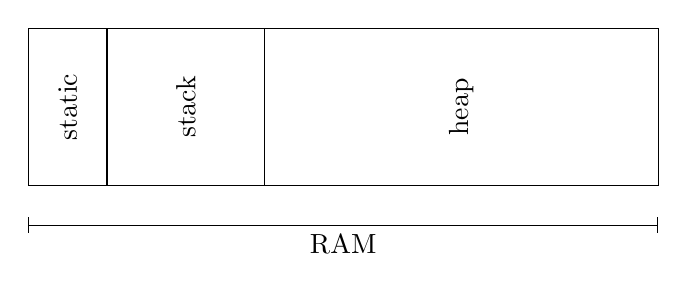
\begin{tikzpicture}
      \draw (0,0) rectangle ++(1,2);
      \draw (1,0) rectangle ++(2,2);
      \draw (3,0) rectangle ++(5,2);

      \node[rotate=90] at (0.5,1) {static};
      \node[rotate=90] at (2,1) {stack};
      \node[rotate=90] at (5.5,1) {heap};

      \draw[|-|] (0,-.5) -- ++(8,0) node[midway,below] {RAM};
    \end{tikzpicture}
  \end{center}
\end{frame}

\begin{frame}
  \frametitle{Heap Allocation}
  \notrealcpp
  \begin{columns}
    \column{5cm}
    \code[font=\small,frame=none,language=c++14]{heap-allocation.cpp}
    \column{4cm}
    \begin{center}
      \begin{tikzpicture}[allocation/.style={-latex,thick},remember picture,overlay,scale=.5]
        \coordinate (start) at (-4,4);

        \only<handout:1-|3->{
          \draw[fill=red!50] (start) rectangle ++(4,-1);
        }
        \only<handout:1|3>{
          \draw[allocation] (var a) to [bend left=30] ($ (start) + (0,-.5) $);
        }

        \only<handout:1-|4->{
          \draw[fill=green!50] ($ (start) + (4,0) $) rectangle ++(4,-1);
        }
        \only<handout:1|4>{
          \draw[allocation] (var b) to [bend left=30] ($ (start) + (4,-0.5) $);
        }

        \only<handout:1-|5->{
          \draw[fill=blue!50] ($ (start) + (0,-1) $) rectangle ++(4,-1);
        }
        \only<handout:1|5>{
          \draw[allocation] (var c) to [bend left=30] ($ (start) + (0,-1.5) $);
        }

        \only<handout:1-|6->{
          \draw[fill=yellow!50] ($ (start) + (4,-1) $) rectangle ++(4,-1);
        }
        \only<handout:1|6>{
          \draw[allocation] (var d) to [bend left=30] ($ (start) + (4,-1.5) $);
        }

        \only<handout:2|7-11>{
          \draw[fill=red!50] ($ (start) + (0,-2) $) rectangle ++(8,-1);
        }
        \only<handout:2|7>{
          \draw[allocation] (mem a) to [bend right=30] ($ (start) + (0,-2.5) $);
        }

        \only<handout:2|8-10>{
          \draw[fill=green!50] ($ (start) + (0,-3) $) rectangle ++(8,-3);
        }
        \only<handout:2|8>{
          \draw[allocation] (mem b) to [bend right=30] ($ (start) + (0,-3.5) $);
        }

        \only<handout:2|9-12>{
          \draw[fill=blue!50] ($ (start) + (0,-6) $) rectangle ++(8,-2);
        }
        \only<handout:2|9>{
          \draw[allocation] (mem c) to [bend right=30] ($ (start) + (0,-6.5) $);
        }

        \only<handout:2|10-13>{
          \draw[fill=yellow!50] ($ (start) + (0,-8) $) rectangle ++(8,-2);
        }
        \only<handout:2|10>{
          \draw[allocation] (mem d) to [bend right=30] ($ (start) + (0,-8.5) $);
        }

        \only<handout:3|11>{
          \draw[->,thick] (del b) ++(2,0) -- ++(-1,0);
        }

        \only<handout:3|12>{
          \draw[->,thick] (del a) ++(2,0) -- ++(-1,0);
        }

        \only<handout:3|13>{
          \draw[->,thick] (del c) ++(2,0) -- ++(-1,0);
        }

        \only<handout:3|14>{
          \draw[->,thick] (del d) ++(2,0) -- ++(-1,0);
        }

        \draw (start) grid ++(8,-10);
      \end{tikzpicture}
    \end{center}
  \end{columns}
  \vskip2cm
  \begin{overprint}
    \onslide<handout:1|2-6>
    \begin{center}
      \textbf{At compile time} \\ Compiler assigns memory locations to each global
    \end{center}

    \onslide<handout:2-3|7->
    \begin{center}
      \textbf{At runtime} \\ Arrays allocated on heap
    \end{center}
  \end{overprint}
\end{frame}

\begin{frame}
  \frametitle{Fragmentation}
  \code[language=c++14]{fragmentation.cpp}
  \begin{center}
    \begin{tikzpicture}[scale=.5]
      \foreach \i in {0,2,...,15} {
        \tikzmath{
          int \j;
          int \k;
          \j = int(\i + 2);
          \k = int(17 + int(\i / 2));
        }
        \only<\j-\k>{
          \draw[fill=red!50] (\i,0) rectangle ++(1,1);
        }
      }

      \foreach \i in {1,3,...,15} {
        \tikzmath{
          int \j;
          \j = int(\i + 2);
        }
        \only<\j-25>{
          \draw[fill=red!50] (\i,0) rectangle ++(1,1);
        }
      }

      \draw (0,0) grid (16,1);
    \end{tikzpicture}
  \end{center}
  \visible<25>{
    \begin{center}
      8 bytes free yet cannot allocate array larger than 1 byte
    \end{center}
  }
\end{frame}

\begin{frame}
  \frametitle{Heap Allocation}
  \begin{procontralist}
    \pro Allows allocation of arbitrarily large blocks
    \pro Deallocation possible in any order
    \pro Most general allocation method
    \con Requires some bookkeeping \\ (keeps track of linked list of free blocks)
    \con Deallocation necessary
    \con Allocation/Deallocation relatively slow
    \con Fragmentation
  \end{procontralist}
\end{frame}


%%% Local Variables:
%%% mode: latex
%%% TeX-master: "allocation-methods"
%%% End:

\begin{frame}
  \frametitle{Garbage Collection}
  \begin{center}
    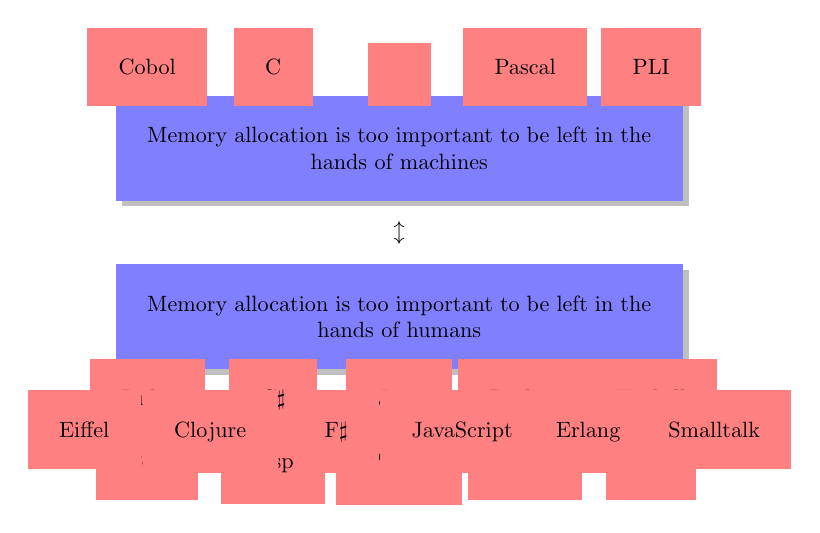
\begin{tikzpicture}[language/.style={fill=red!50},box/.style={fill=blue!50,drop shadow},inner sep=5mm,scale=.8,transform shape]
      \node[anchor=south,box] at (0,.5) {\parbox{8cm}{\centering Memory allocation is too important to be left in the hands of machines}};
      \node at (0,0) {$\updownarrow$};
      \node[anchor=north,box] at (0,-.5) {\parbox{8cm}{\centering Memory allocation is too important to be left in the hands of humans}};

      \visible<2->{
        \node[language,anchor=south] at (0,2) {\cpp};
      }

      \visible<3->{
        \node[language,anchor=north] at (0,-2) {Java};
      }

      \visible<4->{
        \node[language,anchor=south] at (-2,2) {C};
      }

      \visible<5->{
        \node[language,anchor=south] at (2,2) {Pascal};
      }

      \visible<6->{
        \node[language,anchor=south] at (-4,2) {Cobol};
      }

      \visible<7->{
        \node[language,anchor=south] at (4,2) {PLI};
      }

      \visible<8->{
        \node[language,anchor=north] at (-2,-2) {C$\sharp$};
      }

      \visible<9->{
        \node[language,anchor=north] at (2,-2) {Python};
      }

      \visible<10->{
        \node[language,anchor=north] at (-4,-2) {Ruby};
      }

      \visible<11->{
        \node[language,anchor=north] at (4,-2) {Haskell};
      }

      \visible<12->{
        \node[language,anchor=north] at (0,-3) {Prolog};
      }

      \visible<13->{
        \node[language,anchor=north] at (-2,-3) {Lisp};
      }

      \visible<14->{
        \node[language,anchor=north] at (2,-3) {Basic};
      }

      \visible<15->{
        \node[language,anchor=north] at (-4,-3) {Perl};
      }

      \visible<16->{
        \node[language,anchor=north] at (4,-3) {Oz};
      }

      \visible<17->{
        \node[language,anchor=north] at (-1,-2.5) {F$\sharp$};
      }

      \visible<18->{
        \node[language,anchor=north] at (1,-2.5) {JavaScript};
      }

      \visible<19->{
        \node[language,anchor=north] at (-3,-2.5) {Clojure};
      }

      \visible<20->{
        \node[language,anchor=north] at (3,-2.5) {Erlang};
      }

      \visible<21->{
        \node[language,anchor=north] at (-5,-2.5) {Eiffel};
      }

      \visible<22->{
        \node[language,anchor=north] at (5,-2.5) {Smalltalk};
      }
    \end{tikzpicture}
  \end{center}
\end{frame}

\begin{frame}
  \frametitle{Garbage Collection}
  \begin{itemize}
    \item Abstraction of memory
    \item Tries to make it look as if there's an infinite amount of RAM
    \item Recycles unreachable memory
    \item Reduces memory leaks (but does not eliminate them)
    \item Many different techniques
  \end{itemize}
\end{frame}

%%% Local Variables:
%%% mode: latex
%%% TeX-master: "allocation-methods"
%%% End:


\begin{frame}
  \frametitle{Allocation}
  \begin{overprint}
    \onslide<1>
    \begin{center} \Large
      Java
    \end{center}
    \onslide<2>
    \begin{center} \Large
      \cpp
    \end{center}
  \end{overprint}
  \vskip5mm
  \begin{overprint}
    \onslide<1>
    \begin{center}
      \begin{tikzpicture}[static allocation/.style={fill=red!50},
                          stack allocation/.style={fill=blue!50},
                          heap allocation/.style={fill=green!50}]
        \coordinate (o) at (-5,0);
        \coordinate (static) at (o);
        \coordinate (stack) at ($ (o) + (3,0) $);
        \coordinate (heap) at ($ (o) + (6,0) $);

        \draw[static allocation] (o) rectangle ++(3,-4);
        \node[anchor=north,font=\scshape\bfseries] at ($ (static) + (1.5,0) $) {static};

        \draw[stack allocation] (stack) rectangle ++(3,-4);
        \node[anchor=north,font=\scshape\bfseries] at ($ (stack) + (1.5,0) $) {stack};

        \draw[heap allocation] (heap) rectangle ++(3,-4);
        \node[anchor=north,font=\scshape\bfseries] at ($ (heap) + (1.5,0) $) {heap};

        \node[anchor=north west,inner sep=0pt] at ($ (static) + (0,-1) $) {
          \parbox{3cm}{\centering\scshape
            class variables \\
            {\tiny (only primitives)}
          }
        };
        \node[anchor=north west,inner sep=0pt] at ($ (stack) + (0,-1) $) {
          \parbox{3cm}{\centering\scshape
            arguments \\
            locals \\
            {\tiny (only primitives)}
          }
        };
        \node[anchor=north west,inner sep=0pt] at ($ (heap) + (0,-1) $) {
          \parbox{3cm}{\centering\scshape
            object variables
          }
        };
      \end{tikzpicture}
    \end{center}
    \onslide<2>
    \begin{center}
      \begin{tikzpicture}[static allocation/.style={fill=red!50},
                          stack allocation/.style={fill=blue!50},
                          heap allocation/.style={fill=green!50}]
        \coordinate (o) at (-5,0);
        \coordinate (static) at (o);
        \coordinate (stack) at ($ (o) + (3,0) $);
        \coordinate (heap) at ($ (o) + (6,0) $);

        \draw[static allocation] (o) rectangle ++(3,-4);
        \node[anchor=north,font=\scshape\bfseries] at ($ (static) + (1.5,0) $) {static};

        \draw[stack allocation] (stack) rectangle ++(3,-4);
        \node[anchor=north,font=\scshape\bfseries] at ($ (stack) + (1.5,0) $) {stack};

        \draw[heap allocation] (heap) rectangle ++(3,-4);
        \node[anchor=north,font=\scshape\bfseries] at ($ (heap) + (1.5,0) $) {heap};

        \node[anchor=north west,inner sep=0pt] at ($ (static) + (0,-1) $) {
          \parbox{3cm}{\centering\scshape
            globals \\
            class variables \\
            static locals \\
          }
        };
        \node[anchor=north west,inner sep=0pt] at ($ (stack) + (0,-1) $) {
          \parbox{3cm}{\centering\scshape
            arguments \\
            locals
          }
        };
        \node[anchor=north west,inner sep=0pt] at ($ (heap) + (0,-1) $) {
          \parbox{3cm}{\centering\scshape
            anything created with \texttt{new}
          }
        };
      \end{tikzpicture}
    \end{center}
  \end{overprint}
  \vskip5mm
  \begin{overprint}
    \onslide<1>
    \begin{itemize}
      \item Primitives: \texttt{int}, \texttt{boolean}, references, \dots
    \end{itemize}
    \onslide<2>
    \begin{itemize}
      \item Anything can be put anywhere
            \begin{itemize}
              \item Statically allocated objects
              \item Heap allocated \texttt{int}s
              \item \dots
            \end{itemize}
    \end{itemize}
  \end{overprint}
\end{frame}

\begin{frame}
  \frametitle{Allocation Example}
  \begin{center}
    \begin{tikzpicture}[static allocation/.style={fill=red!50},
                        stack allocation/.style={fill=blue!50},
                        heap allocation/.style={fill=green!50},
                        object/.style={drop shadow,draw,fill=white},
                        remember picture]
      \coordinate (o) at (-5,0);
      \coordinate (static) at (o);
      \coordinate (stack) at ($ (o) + (3,0) $);
      \coordinate (heap) at ($ (o) + (6,0) $);

      \draw[static allocation] (o) rectangle ++(3,-4);
      \node[anchor=north,font=\scshape\bfseries] at ($ (static) + (1.5,0) $) {static};

      \draw[stack allocation] (stack) rectangle ++(3,-4);
      \node[anchor=north,font=\scshape\bfseries] at ($ (stack) + (1.5,0) $) {stack};

      \draw[heap allocation] (heap) rectangle ++(3,-4);
      \node[anchor=north,font=\scshape\bfseries] at ($ (heap) + (1.5,0) $) {heap};

      \node[object,anchor=north] (static int 32 bit) at ($ (static) + (1.5,-1)$ ) {32 bits};
    \end{tikzpicture}
  \end{center}
  \code[language=c++14]{int-on-static.cpp}
  \begin{tikzpicture}[remember picture,overlay,allocation/.style={-latex,thick}]
    \codeoverlinex{int on static}
    \draw[allocation] (int on static) -- (static int 32 bit);
  \end{tikzpicture}
\end{frame}

\begin{frame}
  \frametitle{Allocation Example}
  \begin{center}
    \begin{tikzpicture}[static allocation/.style={fill=red!50},
                        stack allocation/.style={fill=blue!50},
                        heap allocation/.style={fill=green!50},
                        object/.style={drop shadow,draw,fill=white},
                        remember picture]
      \coordinate (o) at (-5,0);
      \coordinate (static) at (o);
      \coordinate (stack) at ($ (o) + (3,0) $);
      \coordinate (heap) at ($ (o) + (6,0) $);

      \draw[static allocation] (o) rectangle ++(3,-4);
      \node[anchor=north,font=\scshape\bfseries] at ($ (static) + (1.5,0) $) {static};

      \draw[stack allocation] (stack) rectangle ++(3,-4);
      \node[anchor=north,font=\scshape\bfseries] at ($ (stack) + (1.5,0) $) {stack};

      \draw[heap allocation] (heap) rectangle ++(3,-4);
      \node[anchor=north,font=\scshape\bfseries] at ($ (heap) + (1.5,0) $) {heap};

      \node[object,anchor=north] (stack int 32 bit) at ($ (stack) + (1.5,-1)$ ) {32 bits};
    \end{tikzpicture}
  \end{center}
  \code[language=c++14]{int-on-stack.cpp}
  \begin{tikzpicture}[remember picture,overlay,allocation/.style={-latex,thick}]
    \codeoverlinex{int on stack}
    \draw[allocation] (int on stack) -- (stack int 32 bit);
  \end{tikzpicture}
\end{frame}

\begin{frame}
  \frametitle{Allocation Example}
  \begin{center}
    \begin{tikzpicture}[static allocation/.style={fill=red!50},
                        stack allocation/.style={fill=blue!50},
                        heap allocation/.style={fill=green!50},
                        object/.style={drop shadow,draw,fill=white},
                        remember picture]
      \coordinate (o) at (-5,0);
      \coordinate (static) at (o);
      \coordinate (stack) at ($ (o) + (3,0) $);
      \coordinate (heap) at ($ (o) + (6,0) $);

      \draw[static allocation] (o) rectangle ++(3,-4);
      \node[anchor=north,font=\scshape\bfseries] at ($ (static) + (1.5,0) $) {static};

      \draw[stack allocation] (stack) rectangle ++(3,-4);
      \node[anchor=north,font=\scshape\bfseries] at ($ (stack) + (1.5,0) $) {stack};

      \draw[heap allocation] (heap) rectangle ++(3,-4);
      \node[anchor=north,font=\scshape\bfseries] at ($ (heap) + (1.5,0) $) {heap};

      \node[object,anchor=north] (heap int pointer) at ($ (stack) + (1.5,-1)$ ) {address};
      \node[object,anchor=north] (heap int 32 bit) at ($ (heap) + (1.5,-1)$ ) {32 bits};
    \end{tikzpicture}
  \end{center}
  \code[language=c++14]{int-on-heap.cpp}
  \begin{tikzpicture}[remember picture,overlay,allocation/.style={-latex,thick}]
    \codeoverlinex{int pointer on stack}
    \codeoverlinex{int on heap}
    \draw[allocation] (int pointer on stack) -- (heap int pointer);
    \draw[allocation] (int on heap) -- (heap int 32 bit);
  \end{tikzpicture}
\end{frame}

\begin{frame}
  \frametitle{Allocation}
  \begin{itemize}
    \item Same applies on \emph{all} types
    \item Same treatment for both primitives and objects
    \item For example, objects can be put on stack
  \end{itemize}

  \code[language=c++14]{object-on-stack.cpp}
\end{frame}

\end{document}


%%% Local Variables:
%%% mode: latex
%%% TeX-master: "allocation-methods"
%%% End:
